Presentamos gráficamente los datos recogidos en la figura (\ref{figure_difractogramas}).

\begin{figure*}[t]
	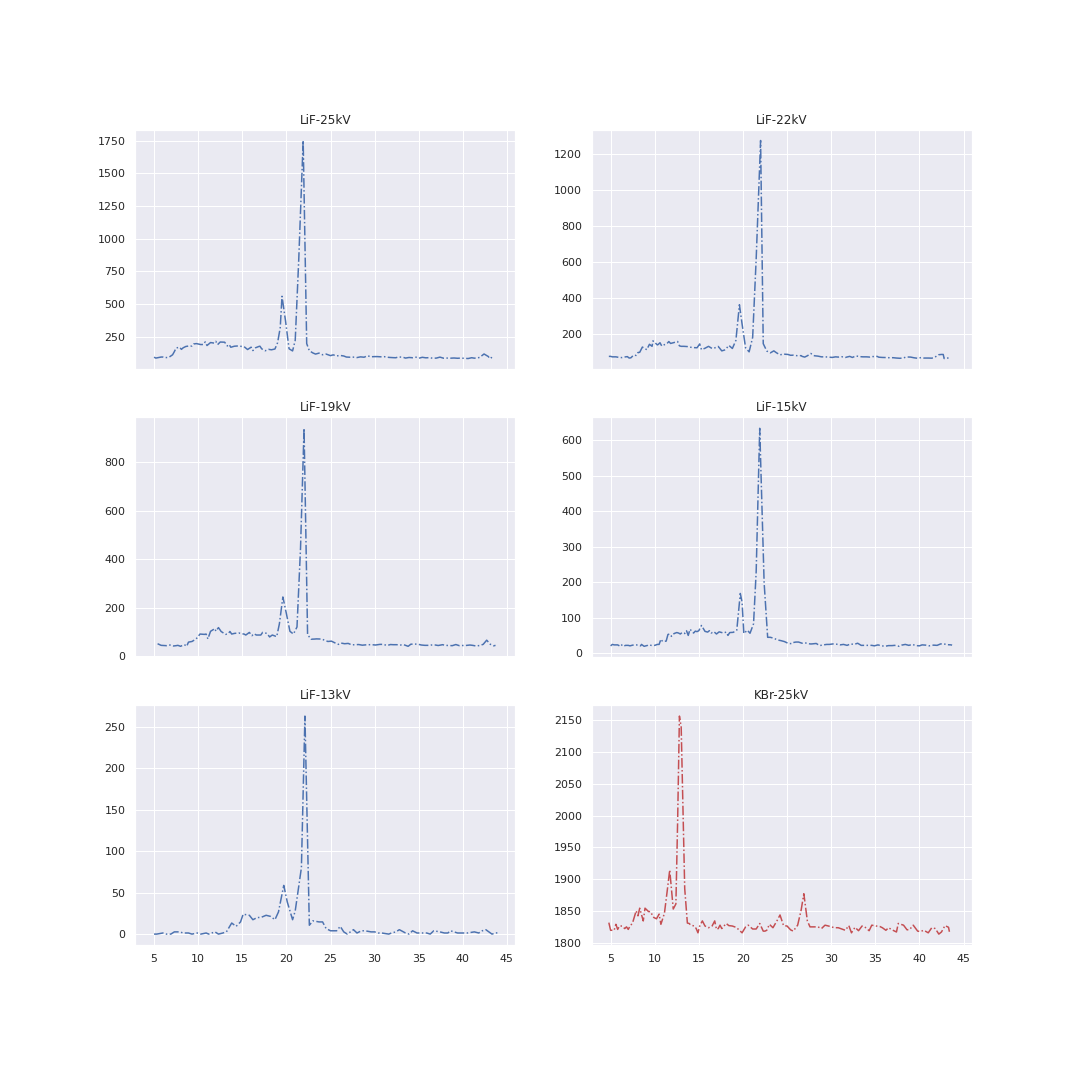
\includegraphics[width=\linewidth,height=20cm]{difractogramas}
	\caption{Difractogramas de rayos X con energías comprendidas entre 13 y 25 kV}
	\label{figure_difractogramas}
\end{figure*}

\subsection{LiF}

Los datos de ángulos para las cinco medidas los podemos ver en la tabla (\ref{table_angulos}). Como podemos ver en dicha tabla, al aumentar la tensión también aumenta la intensidad de los picos del LiF, siempre para los mismos ángulos. Con los datos para las transiciones energéticas de la figura (\ref{figure_radiacion_cobre}) y la media de los datos de la tabla (\ref{table_angulos}) tenemos que el pico para la transición $K_{\alpha1,2}=8037.5$kV se consigue para un ángulo (medio) $21.98 \pm 0.07$(º) mientras que para la transición $K_{\beta}=8902$kV corresponde un ángulo de $19.62 \pm 0.07$(º)

\begin{table*}[t]
	\centering
	\begin{tabular}{ccccc}
		\toprule
		\multicolumn{1}{c}{} & \multicolumn{2}{c}{$K_{\beta}$} & \multicolumn{2}{c}{$K_{\alpha}$} \\
		\cmidrule(r){2-5}
		& Ángulo (ª)    & Intensidad    & Ángulo (ª) & Intensidad \\
		\midrule
		LiF 13kV & $19.7 \pm 0.1$    & 58.67    & $22.1 \pm 0.1$ & 262.67 \\
		LiF 15kV & $19.7 \pm 0.1$    & 168.67    & $21.9 \pm 0.1$ & 633.33 \\
		LiF 19kV & $19.6 \pm 0.1$    & 244.0    & $22.0 \pm 0.1$ & 941.33 \\
		LiF 22kV & $19.6 \pm 0.1$    & 361.33    & $22.0 \pm 0.1$ & 1277.33 \\
		LiF 25kV & $19.5 \pm 0.1$    & 560.0    & $21.9 \pm 0.1$ & 1750.0 \\
		KBr 25kV (1º) & $11.7 \pm 0.1$    & 1914.67    & $12.8 \pm 0.1$ & 2156.0 \\
		KBr 25kV (2º) & $24.2 \pm 0.1$    & 1844.0    & $26.9 \pm 0.1$ & 1877.33 \\
		\bottomrule
	\end{tabular}
	\caption{Ángulos para los picos $K_{\alpha}$ y $K_{\beta}$}
	\label{table_angulos}
\end{table*}

Gracias a estos datos y haciendo uso de la ecuación (\ref{eq_distancia}) con $n=1$ dado que estos picos de intensidad corresponden al primer orden de difracción llegamos a que la distancia interplanar (en valor medio) es $d = (2.06 \pm 0.05)\cdot 10^{-10}$m. 

Conocido el valor de la distancia interplanar, podemos ver que la condición que deben satisfacer los índices de Miller del conjunto de planos involucrados en la difracción es $ h^2 + k^2 + l^2 \approx 4$. La única posibilidad es considerar el conjunto de planos (2,0,0), (0,2,0) o (0,0,2) y por lo tanto el parámetro de red experimental será $a = 2d = (4.12 \pm 0.10)\cdot 10^{-10}$m, un 2\% superior al valor teórico.

Para determinar experimentalmente el valor de la constante de Planck debemos hacer uso de la ecuación (\ref{eq_angulo_min}) donde el ángulo mínimo $\theta_{min}$ será aquel ángulo para el que empieza a ser apreciable la radiación de frenado, caracterizada por un espectro continuo que hace de "baseline" en nuestro conjunto de datos. Los datos y su correspondiente regresión lineal los podemos ver en la figura (\ref{figure_planck}). El valor de $R^2$ es relativamente bajo debido a que se ha seleccionado el valor de $\theta_{min}$ por inspección visual. Podemos identificar entonces la pendiente de la regresión lineal como $\frac{hc}{2de}$, de tal manera que al despejar y sustituir obtenemos $h = (5.5 \pm 0.9)\cdot 10^{-34} J \cdot s$

\begin{figure}[H]
	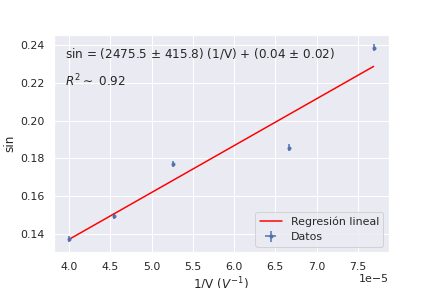
\includegraphics[width=\linewidth]{planck}
	\caption{Seno del ángulo (mínimo) a partir del cual empieza a salir radiación de frenado}
	\label{figure_planck}
\end{figure}

\subsection{KBr}

Igualemnte que para el caso del LiF, podemos ver los datos en la figura (\ref{figure_radiacion_cobre}) y la tabla (\ref{table_angulos}). En este caso podemos ver los picos de segundo orden en la figura del difractograma. Llevado a cabo los mismos cálculos tenemos, siendo la media correspondiente a los cuatro picos, $d = (3.43 \pm 0.11)\cdot 10^{-10}$m y por lo tanto $a = 2d = (6.9 \pm 0.2)\cdot 10^{-10}$m. En este caso el parámetro de red es un 4\% superior al valor teórico.